\documentclass[tikz,border=2pt]{standalone}
\usepackage{xcolor}
\usetikzlibrary{arrows.meta,positioning}

\definecolor{ink}{HTML}{26363E}
\definecolor{muted}{HTML}{667781}
\definecolor{teal}{HTML}{167F78}
\definecolor{tealbg}{HTML}{EDF7F5}
\definecolor{blue}{HTML}{3973B7}
\definecolor{bluebg}{HTML}{EEF4FA}
\definecolor{orange}{HTML}{C97820}
\definecolor{orangebg}{HTML}{FFF4E7}
\definecolor{blocked}{HTML}{88969C}

\begin{document}
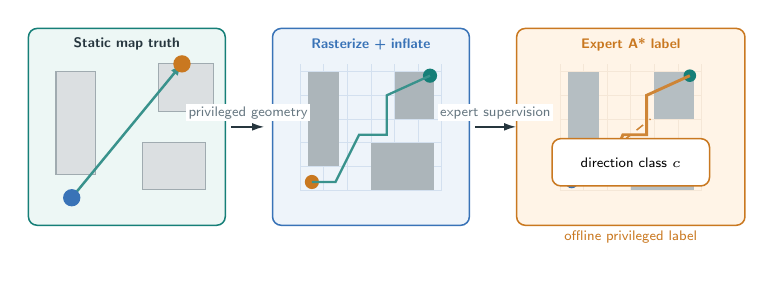
\begin{tikzpicture}[
  x=1mm,y=1mm,font=\sffamily,
  box/.style={rounded corners=1.1mm,line width=.55pt,align=center,inner sep=1.1mm},
  title/.style={font=\sffamily\bfseries\fontsize{5.4}{6.1}\selectfont,
                text=ink,align=center},
  sub/.style={font=\sffamily\fontsize{3.8}{4.4}\selectfont,
              text=muted,align=center},
  tiny/.style={font=\sffamily\fontsize{3.25}{3.8}\selectfont,
               text=muted,align=center},
  flow/.style={-{Latex[length=1.6mm,width=1mm]},line width=.75pt,draw=ink}
]

% 1. Privileged static geometry.
\node[box,draw=teal,fill=tealbg,minimum width=25mm,minimum height=25mm]
  (truth) at (13,15) {};
\node[title] at (13,25.5) {Static map truth};
\draw[draw=blocked!80,fill=blocked!30] (4,9)--(9,9)--(9,22)--(4,22)--cycle;
\draw[draw=blocked!80,fill=blocked!30] (15,7)--(23,7)--(23,13)--(15,13)--cycle;
\draw[draw=blocked!80,fill=blocked!30] (17,17)--(24,17)--(24,23)--(17,23)--cycle;
\draw[teal!85,line width=.9pt,-{Latex[length=1.5mm]}] (6,6)--(20,23);
\fill[blue] (6,6) circle (1.1mm);
\fill[orange] (20,23) circle (1.1mm);

% 2. Rasterization and vehicle inflation.
\node[box,draw=blue,fill=bluebg,minimum width=25mm,minimum height=25mm]
  (grid) at (44,15) {};
\node[title,text=blue] at (44,25.5) {Rasterize + inflate};
\foreach \x in {35,38,41,44,47,50,53} {\draw[blue!22,line width=.25pt] (\x,7)--(\x,23);}
\foreach \y in {7,10,13,16,19,22} {\draw[blue!22,line width=.25pt] (35,\y)--(53,\y);}
\fill[blocked!70] (36,10) rectangle (40,22);
\fill[blocked!70] (44,7) rectangle (52,13);
\fill[blocked!70] (47,16) rectangle (52,22);
\fill[orange] (36.5,8) circle (.9mm);
\fill[teal] (51.5,21.5) circle (.9mm);
\draw[teal!85,line width=.85pt] (36.5,8)--(39.5,8)--(42.5,14)--(46,14)--(46,19)--(51.5,21.5);

% 3. Expert route and direction label.
\node[box,draw=orange,fill=orangebg,minimum width=29mm,minimum height=25mm]
  (astar) at (77,15) {};
\node[title,text=orange] at (77,25.5) {Expert A* label};
\foreach \x in {68,71,74,77,80,83,86} {\draw[orange!18,line width=.25pt] (\x,7)--(\x,23);}
\foreach \y in {7,10,13,16,19,22} {\draw[orange!18,line width=.25pt] (68,\y)--(86,\y);}
\fill[blocked!62] (69,10) rectangle (73,22);
\fill[blocked!62] (77,7) rectangle (85,13);
\fill[blocked!62] (80,16) rectangle (85,22);
\fill[blue] (69.5,8) circle (.8mm);
\fill[teal] (84.5,21.5) circle (.8mm);
\draw[orange!90,line width=1.05pt] (69.5,8)--(73.5,8)--(76,14)--(79,14)--(79,19)--(84.5,21.5);
\draw[orange!90,line width=.55pt,dashed] (69.5,8)--(79.5,16);
\node[box,draw=orange,fill=white,minimum width=20mm,minimum height=6mm]
  at (77,10.5) {\fontsize{4.0}{4.5}\selectfont direction class $c$};

\draw[flow] (26.2,15)--(30.5,15);
\draw[flow] (57.2,15)--(62.5,15);
\node[tiny,fill=white,inner sep=.3mm] at (28.4,16.8) {privileged geometry};
\node[tiny,fill=white,inner sep=.3mm] at (59.8,16.8) {expert supervision};
\node[tiny,text=orange] at (77,1.0) {offline privileged label};

\end{tikzpicture}
\end{document}
